\documentclass[11pt, a4paper]{article}
\usepackage[english]{babel}
\usepackage[utf8]{inputenc}
\usepackage{hyperref}
\usepackage{graphicx}
\usepackage{array}
\usepackage{enumitem}
\usepackage{pifont}
\usepackage{threeparttable}
\usepackage{amsmath}
\usepackage{booktabs}
\usepackage{fancyhdr}
\usepackage{pdflscape}

\renewcommand{\arraystretch}{1.5}

\graphicspath{ {./images/} }
\bibliographystyle{plain}

\title{ \Huge{Research report: \\ Prosthetic hand} \\ \vspace{1cm} \normalsize{\textit{First iteration}}} 
\author{Written by: \\ Dylan Duunk \textit{(0948392)} \\ \textit{Discipulus-Ex} 
\vspace{1cm} \\
Written for: \\ Ornella Schavemaker-Piva, \\ Wouter Volders \& \\ Nadine van Dormolen}
\vspace{1cm}
\date{12th April 2019}

\begin{document}

\begin{titlepage}
    \maketitle
\end{titlepage}

\pagenumbering{roman}

\newpage
 
\begin{abstract}
    \noindent
    Contemporary prostheses have advanced significantly the last few years.
    Previously, prostheses were quite expensive, nowadays one can 3D print a open-source prosthesis design.
    Unfortunately those designs are mostly made for below-elbow and above-elbow amputees.
    Our audience are people with a partial hand.
    With a partial hand prosthesis you also have to take the length of the user's arm in account.
    This makes it difficult to design prostheses for them.
    \\ \\
    So the research question is as follows: 
    \emph{
        \vspace{5pt}
        \begin{center}
            ``How to make an efficient design for a partial hand prosthesis and which parts are involved in making such a design?''
        \end{center}
        \vspace{5pt}
    }
    
    \noindent
    In this research report I will describe the different factors that play a role in making a prosthesis design, such as material choice and comfort.
    Furthermore I will describe the design I came up with.
\end{abstract}    

\newpage
\tableofcontents
\newpage
\pagenumbering{arabic}

\pagestyle{fancy}
\fancyhf{}
\rhead{Dylan Duunk}
\lhead{Research report: Prosthetic hand}
\rfoot{\thepage}

\section{Introduction}
Prostheses have advanced significantly in their functional capabilities and appearances over the past few years.
The latest trends in fabrication are elevating prosthetic comfort, function and appearance for thousands of prosthesis users.
But most of the higher-end prostheses are way to expensive for most people, while more and more people are eligible for prostheses.
\\ \\
With the latest technology of 3D printing and greater access to a 3D printer, the production of prostheses has become a lot easier and cheaper.
With the open source community of 3D printing, everyone with access to a 3D printer can make a prosthesis for themselves or for others.
\\ \\
Unfortunately for people with a partial hand, there are barely any designs for partial hand prostheses.
Most of these designs are body-powered prostheses or finger prostheses.
\\ \\
In this document, I will assess a variety of materials based on their suitability for prostheses whilst maintaining a comfortable fit and I show my design for a partial hand prosthesis and the idea behind it.

\section{Preliminary investigation}
One of the earliest records of a prosthetic hand was described n 77 AD by Roman scholar Pliny the Elder in his encyclopedia \textit{Naturalis Historia}\cite{natural_history}.
After losing a hand in the Second Punic War (218-201 BC), Marcus Sergius, a Roman general, received a prosthesis that enabled him to return successfully to battle and continue his position as a general.
\\ \\ 
Among the most famous example of an early hand prosthesis was the iron hand of German knight G\"otz von Berlichtingen \cite{historical_prostheses}.
After G\"otz lost his hand during the Siege of Landshut (circa 1505) in Bavaria, an artisan fashioned him an iron hand with digits that could be flexed and extended passively at finger joints (Figure \ref{fig:GotzProsthesis}).
Due to its weight, the device needed to be attached to G\"otz armour rather than his arm. 
\\
\begin{figure}[h]
    \centering
    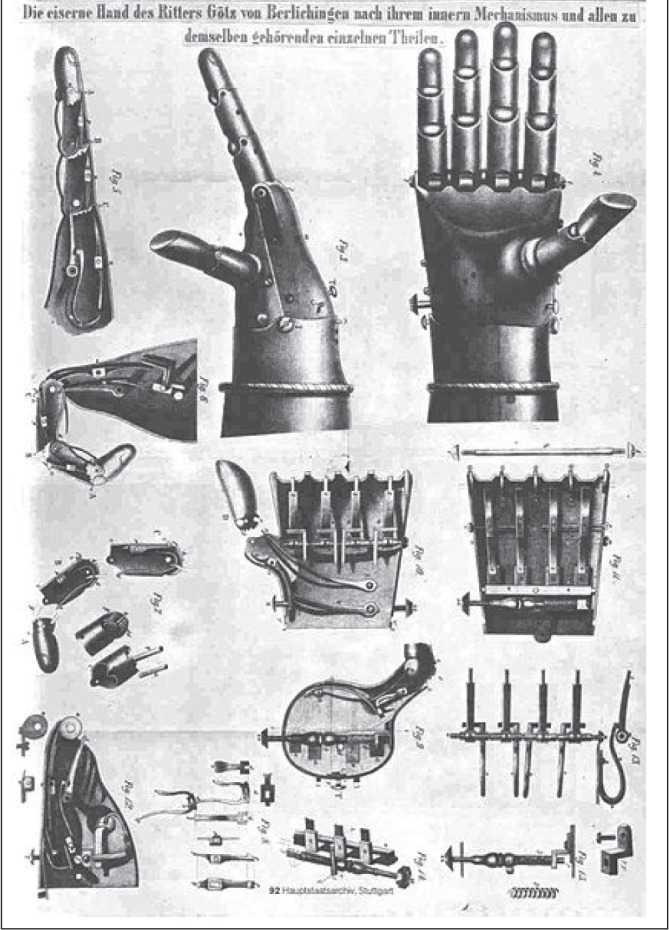
\includegraphics[scale=0.26]{GotzProsthesis.jpg}
    \caption{Illustration of the numerous components of G\"otz's medieval hand prosthesis.}
    \label{fig:GotzProsthesis}
\end{figure}

\newpage

\noindent 
The concept of an body-powered upper limb prosthesis was pioneered by German dentist Peter Baliff in 1818 \cite{history_of_arm_amputation}.
Using transmission of tension through leather straps.
Baliff's device was opperated by the use of the trunk and shoulder girdle to elicit motion in the device.
\\ \\
In 1916, German surgeon Dr Ferdinand Sauerbruch described his prosthetic design with digits controlled by transmission of upper arm muscle movements (Figure \ref{fig:SauerbrunchProsthesis}) \cite{sauerbrunch}.
Unfortunately, due to the high cost of production, few individuals were able to afford the device.
\\
\begin{figure}[h]
    \centering
    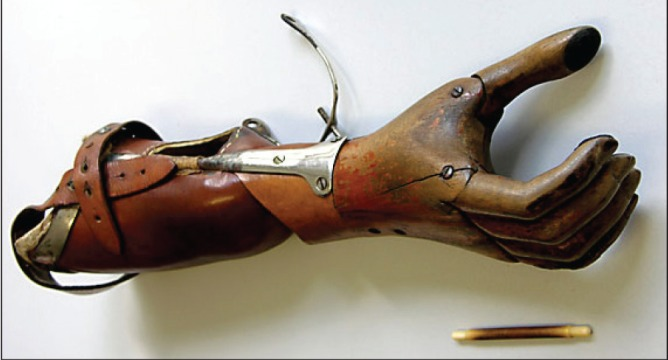
\includegraphics[scale=0.23]{SauerbrunchProsthesis.jpg}
    \caption{Sauerbrunch's prosthetic hand design. Video captures of patients using the prosthesis to perform various activities may by viewed at \url{http://vlp.mpiwg-berlin.mpg.de/library/data/lit38416}}
    \label{fig:SauerbrunchProsthesis}
\end{figure} 

\noindent
In 1948, the Bowden cable body-powered prosthesis was introduced, replacing bulky straps with a sleek, sturdy cable.
Today's body-powered prostheses are essentially adaptations of the Bowden design (Figure \ref{fig:BowdenProsthesis}). 
Durable, portable and relatively affordable, body-powered prostheses allow the user an impressive range of motion, speed and force in operating a terminal device.
This design works by changing the tension in a cable via shoulder and body movements.
The design allows the ability to use both hands simultaneously, rather that requiring a healthy hand to control the prosthesis.
Furthermore, the user is able to predict and adjust the position of the prosthesis without visual feedback.
Although prolonged wearing can be uncomfortable, complicated motor tasks are limited and appearance is not human-like, body-powered prostheses are widely used.
\\
\begin{figure}[h]
    \centering
    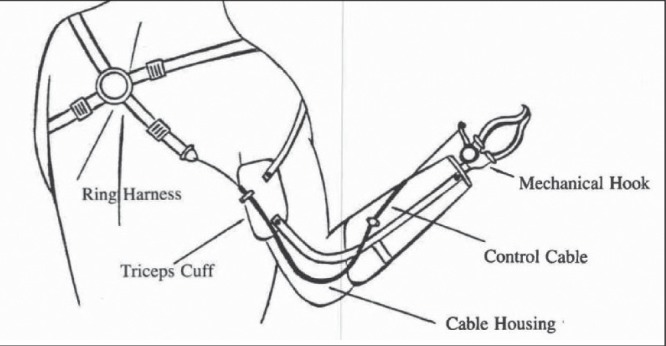
\includegraphics[scale=0.4]{BowdenProsthesis.jpg}
    \caption{Bowden cable body powered prosthesis.}
    \label{fig:BowdenProsthesis}
\end{figure} 

\noindent
In 1919, a German book titled \textit{Ersatzglieder un Arbeitshilfen (Limb Substitutes and Work Aids)} contained conceptual designs for the first externally powered prostheses, using pneumatic and electric power sources (Figure \ref{fig:PrebluftHand}).
Unfortunately, these revolutionary designs were to complex for their time.
\\
\begin{figure}[h]
    \centering
    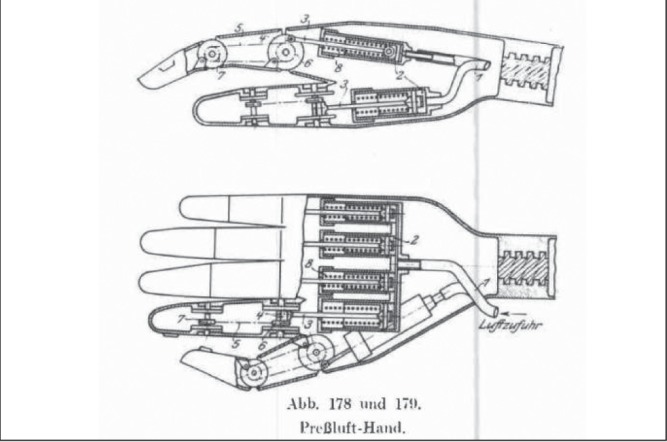
\includegraphics[scale=0.4]{PrebluftHand_1.jpg}
    \caption{Early compressed gas-powered prosthetic hand from 1919 German book \textit{Ersatzglieder un Arbeitshilfen (Limb Substitutes and Work Aids)}.}
    \label{fig:PrebluftHand}
\end{figure} 

\noindent
The first myoelectric prosthesis was created in 1948 by Reinhold Reiter, a physics student at Munich University (Munich, Germany).
This device amplifies surface electromyography (EMG) potentials to power motorized parts.
\\ \\
The first clinically significant myoelectric prosthesis was unveiled by Russian scientist Alexander Kobrinski in 1960.
With the use of transistors he managed to reduce bulk and allowed portability of the prosthesis.
This prosthesis had numerous problems: it was heavy, movement was slow, pinch force was weak, wire connections were susceptible to damage and electrical interference compromised reliability \cite{myoelectric}.  

\newpage

\noindent
Nowadays myoelectric prostheses are a common option for amputees. 
They improved drastically in design, weight, power and cost.
In addition, signal detection is noninvasive on the skin surface and prosthetic movement is comparable with a normal limb.

\begin{figure}[h]
    \centering
    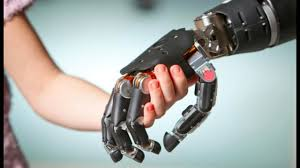
\includegraphics[scale=0.7]{HeroArm.jpg}
    \caption{The Hero Arm, the world's first medically certified 3D-printed bionic arm, with multi-grip functionality and empowering aesthetics. \textit{Developed by OpenBionics} \url{https://openbionics.com/hero-arm/}}
    \label{fig:HeroArm}
\end{figure}    

\noindent
The problem with contemporary myoelectric prostheses is that they are primarily made for below-elbow and above-elbow amputees.
For our version we need to make a prosthetic hand for someone with a partial hand and therefore cannot use these common myoelectric prostheses.
So we need to come up with our own design.
\\ \\
This design needs to incorporate a lightweight material and has to be comfortable to use.

\section{Methodology}
My research consists of three parts: material, comfort and a prototype design incorporating the two previous aspects.
\\
These are my research methods for each part:
\begin{description}[align=left]
    \item[Material] Review a variety of commonly used materials for prostheses and compare them to each other.
    \item[Comfort] Research which factors play a role in comfort.
    \item[Prototype design] Experiment with various designs.
\end{description}    

\section{Results}
These are the results of my research:
\subsection{Materials} \label{materials}
Material choice plays a major role in prostheses.
Prostheses must be both strong and lightweight, they must be able to withstand the extensive use of the owner without obstructing there range of motion.
\\
Below I will review a variety of materials for our prosthetic hand.

\subsubsection{Plastic}
PLA and ABS are 2 of the most common FDM (Fused deposition modeling) desktop printing materials.
Both materials are thermoplastics, meaning they become pliable or moldable at a certain elevated temperature and solidifies upon cooling.
Via the FDM process, both materials are melted and then extruded trough a nozzle to build up the layers that create a final part.
\\ \\
Table \ref{tab:pla-abs} below compares the main properties between PLA \& ABS:

\begin{table}[ht]
    \centering
    \begin{threeparttable}
        \begin{tabular}[t]{>{\bfseries}l l l}
            \toprule
            Properties\tnote{1} & \textbf{PLA} & \textbf{ABS} \\
            \midrule
            Density & $1.3 g/cm^3$ & $1.0 - 1.4 g/cm^3$ \\
            Elongation & 6\% & 3.5-50\% \\ %https://en.wikipedia.org/wiki/Deformation_(mechanics)#Stretch_ratio
            Flexural Modulus & 4GPa & 2.1-7.6 GPa \\ %https://en.wikipedia.org/wiki/Flexural_modulus
            Melting Point & $160\,^{\circ}{\rm C}$ & N/A (amorphous) \\
            Biodegradable & Yes, under the correct conditions & No \\
            Glass Transition Temperature & $60\,^{\circ}{\rm C}$ & $105\,^{\circ}{\rm C}$ \\ %https://en.wikipedia.org/wiki/Glass_transition
            \bottomrule
        \end{tabular}
        \caption{Comparing PLA with ABS}
        \label{tab:pla-abs}
        \begin{tablenotes}
            \item[1] \textit{Sourced from MakeItFrom \cite{MakeItFrom}}
        \end{tablenotes}    
    \end{threeparttable}    
\end{table}

\subsubsection{Silicone}
Silicone is a dynamic material that moves with the body while simultaneously offering 
an enhanced grip on the residual limb and improved suspension of the prosthesis.
Silicone is mostly used in realistic looking prosthetics and for mold making.
\\ \\ 
Table \ref{tab:silicone-properties} below gives the main properties of silicone:

\begin{table}[ht]
    \centering
    \begin{threeparttable}
        \begin{tabular}[t]{>{\bfseries}l l}
            \toprule
            Properties\tnote{1} & \textbf{Silicone plastic}  \\
            \midrule
            Density & $1.9 g/cm^3$  \\
            Elastic Modulus & 9.0 GPa \\ %https://en.wikipedia.org/wiki/Elastic_modulus
            Max. Temperature: Decomposition & $480\,^{\circ}{\rm C}$  \\
            Biodegradable & No  \\
            Glass Transition Temperature & $200\,^{\circ}{\rm C}$  \\ %https://en.wikipedia.org/wiki/Glass_transition
            \bottomrule
        \end{tabular}
        \caption{Properties silicone plastic}
        \label{tab:silicone-properties}
        \begin{tablenotes}
            \item[1] \textit{Sourced from MakeItFrom \cite{MakeItFrom}}
        \end{tablenotes}    
    \end{threeparttable}    
\end{table}

\subsubsection{Carbon Fiber}
Carbon fiber reinforced plastic (CFRP), is an extremely strong and light fiber-reinforced plastic which contains carbon fibers.
Carbon fiber is often used in prosthetics, sports equipment, aerospace and wherever the high strength-to-weight ratio and stiffness from carbon fiber are required.
CFRPs are composite materials.
In this case the composite consists of two parts: a matrix and a reinforcement.
In this case the reinforcement is carbon fiber, which provides the strength.
The matix is usually a polymer resin, such as epoxy, to bind the reinforcements together.
This makes the material properties depend on those distinct elements.

\subsubsection{Metal}
Alloys containing titanium are known for their high strength, lightweight, and exceptional corrosion resistance.
Despite being as strong as steel, titanium is about 40\% lighter in weight.
Titanium is also formidable in its resistance to corrosion by both water and chemical media.
\\
Because titanium has a low modulus of elasticity that means titanium is not also very flexible, but returns to its original shape after bending.
\\ \\
Aluminium is a very light metal with a specific weight of $2.7 g/cm^3$, about a third that of steel.
Its strength can be adapted to the apllication required by modifying the composition of its alloys.
Aluminium naturally generates a protective oxide coating and is highly corrosion resistant which can be further imporeved by different types of surface treatments. 
This is particularly usefull for applications where protection and conservation are required.

\subsubsection{Morphological chart}

\begin{table}[ht]
    \centering
    \begin{threeparttable}
        \begin{tabular}[t]{>{\bfseries}l c c c c c c}
            \toprule
            & \textbf{PLA} & \textbf{ABS} & \textbf{Silicone} & \textbf{Carbon} & \textbf{Titanium\tnote{1}} & \textbf{Aluminium\tnote{1}}  \\
            \midrule
            Easy of use & \ding{72}\ding{72}\ding{72}\ding{72}\ding{72} & \ding{72}\ding{72}\ding{72}\ding{72}\ding{73} & \ding{72}\ding{72}\ding{72}\ding{73}\ding{73} & \ding{72}\ding{72}\ding{73}\ding{73}\ding{73} & \ding{72}\ding{73}\ding{73}\ding{73}\ding{73} & \ding{72}\ding{72}\ding{73}\ding{73}\ding{73} \\
            Strength & \ding{72}\ding{72}\ding{73}\ding{73}\ding{73} & \ding{72}\ding{72}\ding{72}\ding{73}\ding{73} & \ding{72}\ding{72}\ding{72}\ding{72}\ding{73} & \ding{72}\ding{72}\ding{72}\ding{72}\ding{72} & \ding{72}\ding{72}\ding{72}\ding{72}\ding{72} & \ding{72}\ding{72}\ding{72}\ding{72}\ding{72} \\
            Weight\tnote{2} & \ding{72}\ding{72}\ding{72}\ding{72}\ding{72} & \ding{72}\ding{72}\ding{72}\ding{72}\ding{72}  & \ding{72}\ding{72}\ding{72}\ding{72}\ding{72} & \ding{72}\ding{72}\ding{72}\ding{72}\ding{72} & \ding{72}\ding{72}\ding{72}\ding{72}\ding{72} & \ding{72}\ding{72}\ding{72}\ding{72}\ding{72}  \\
            Elastic Modulus & \ding{72}\ding{72}\ding{73}\ding{73}\ding{73} & \ding{72}\ding{72}\ding{72}\ding{73}\ding{73} & \ding{72}\ding{72}\ding{72}\ding{72}\ding{72} & \ding{72}\ding{72}\ding{72}\ding{73}\ding{73} & \ding{72}\ding{72}\ding{72}\ding{72}\ding{72} & \ding{72}\ding{72}\ding{72}\ding{73}\ding{73} \\
            Price & \ding{72}\ding{72}\ding{72}\ding{72}\ding{72} & \ding{72}\ding{72}\ding{72}\ding{72}\ding{72} & \ding{72}\ding{72}\ding{72}\ding{72}\ding{73} & \ding{72}\ding{72}\ding{73}\ding{73}\ding{73} & \ding{72}\ding{73}\ding{73}\ding{73}\ding{73} & \ding{72}\ding{72}\ding{72}\ding{73}\ding{73} \\
            Usability\tnote{3} & \ding{72}\ding{72}\ding{72}\ding{72}\ding{72} & \ding{72}\ding{72}\ding{72}\ding{72}\ding{73} & \ding{72}\ding{72}\ding{72}\ding{73}\ding{73} & \ding{72}\ding{73}\ding{73}\ding{73}\ding{73} & \ding{73}\ding{73}\ding{73}\ding{73}\ding{73} & \ding{72}\ding{73}\ding{73}\ding{73}\ding{73} \\
            \bottomrule
        \end{tabular}
        \caption{Materials Morphological Chart}
        \label{tab:morphchart-material}  
        \begin{tablenotes}
            \item[] These values in this Morphological Chart are based on eachother.
            \item[1] The material properties of these materials can vary based on the alloys used.
            \item[2] Weight is based on how lightweight the material is.
            \item[3] Usability in this case is based on how usefull this material will be for our prototype.  
        \end{tablenotes}    
    \end{threeparttable}   
\end{table}

\subsection{Comfort}
Comfort is an important factor for prostheses.
The prostheses must be an addition for the user, so that the user benefits of the prosthetic instead of being a chore.
Ideally the user shouldn't notice that a prosthesis is present.
This makes the user feel like a normal person and that the prosthesis is part of the body.
\\
Below I will describe which factors play a role in the comfort of prostheses.

\begin{description}[align=left]
    \item[Weight] The user must be able to wear the prosthesis for long periods of time in order to be usefull, this is why the prosthesis must be lightweight.
                  Otherwise the user has to carry the have load of the prosthesis and is therefore not sufficient.
    \item[Range of motion] The user must be able to have a relatively free range of motion, so that the user doesn't feel restricted.                       
    \item[Fit] The prosthesis must be securly fit to the user without impending the bloodflow.
               The fit shouldn't be to loose either, otherwise it will slip around all the time. 
    \item[Breathability] Because the user is wearing the prosthesis for longer periods of time, the user's skin needs to be able to freely breathe.   
    \item[Aesthetics] For some people the prosthesis my not stand out.
                      The attention some people get with a prosthesis may be annoing sometimes. 
\end{description}

\subsection{Prototype Design}
\textit{*Note: So far, the prototype only consists of the connection between my (Dylan) arm and a potential hand}

\subsubsection{First Prototype}
For the first prototype I wanted to make a casing for my forearm.
Because I didn't have access to a 3D scanner I had to come up with another solution to convert my drawings (Figure \ref{fig:ConceptPrototype1}) into a 3D model.
So I took measurements of my arm at different points, and seperated them into circles.
With these circles I moddeled around those circles in Fusion 360 and came up with this design (Figure \ref{fig:Prototype1Mechanical}). 
\\ \\
See table \ref{tab:FirstPrototypeProsCons} for the pros and cons of the first prototype.
\begin{table}[ht]
    \centering
    \begin{tabular}[t]{p{6cm} p{6cm}}
    \toprule
    \textbf{Pros} & \textbf{Cons} \\
    \midrule
    Thickness of the prototype is good. & For a someone with a partial hand this design is unneccessary bulky. \\
    & Design is more suitable for below-elbow amputees. \\
    & Fit was to small in diameter, which was solved by heating the prototype in hot water and reforming it. \\
    \bottomrule
    \end{tabular}
    \caption{First Prototype: Pros \& Cons}
    \label{tab:FirstPrototypeProsCons}
\end{table}

\begin{figure}[h]
    \centering
    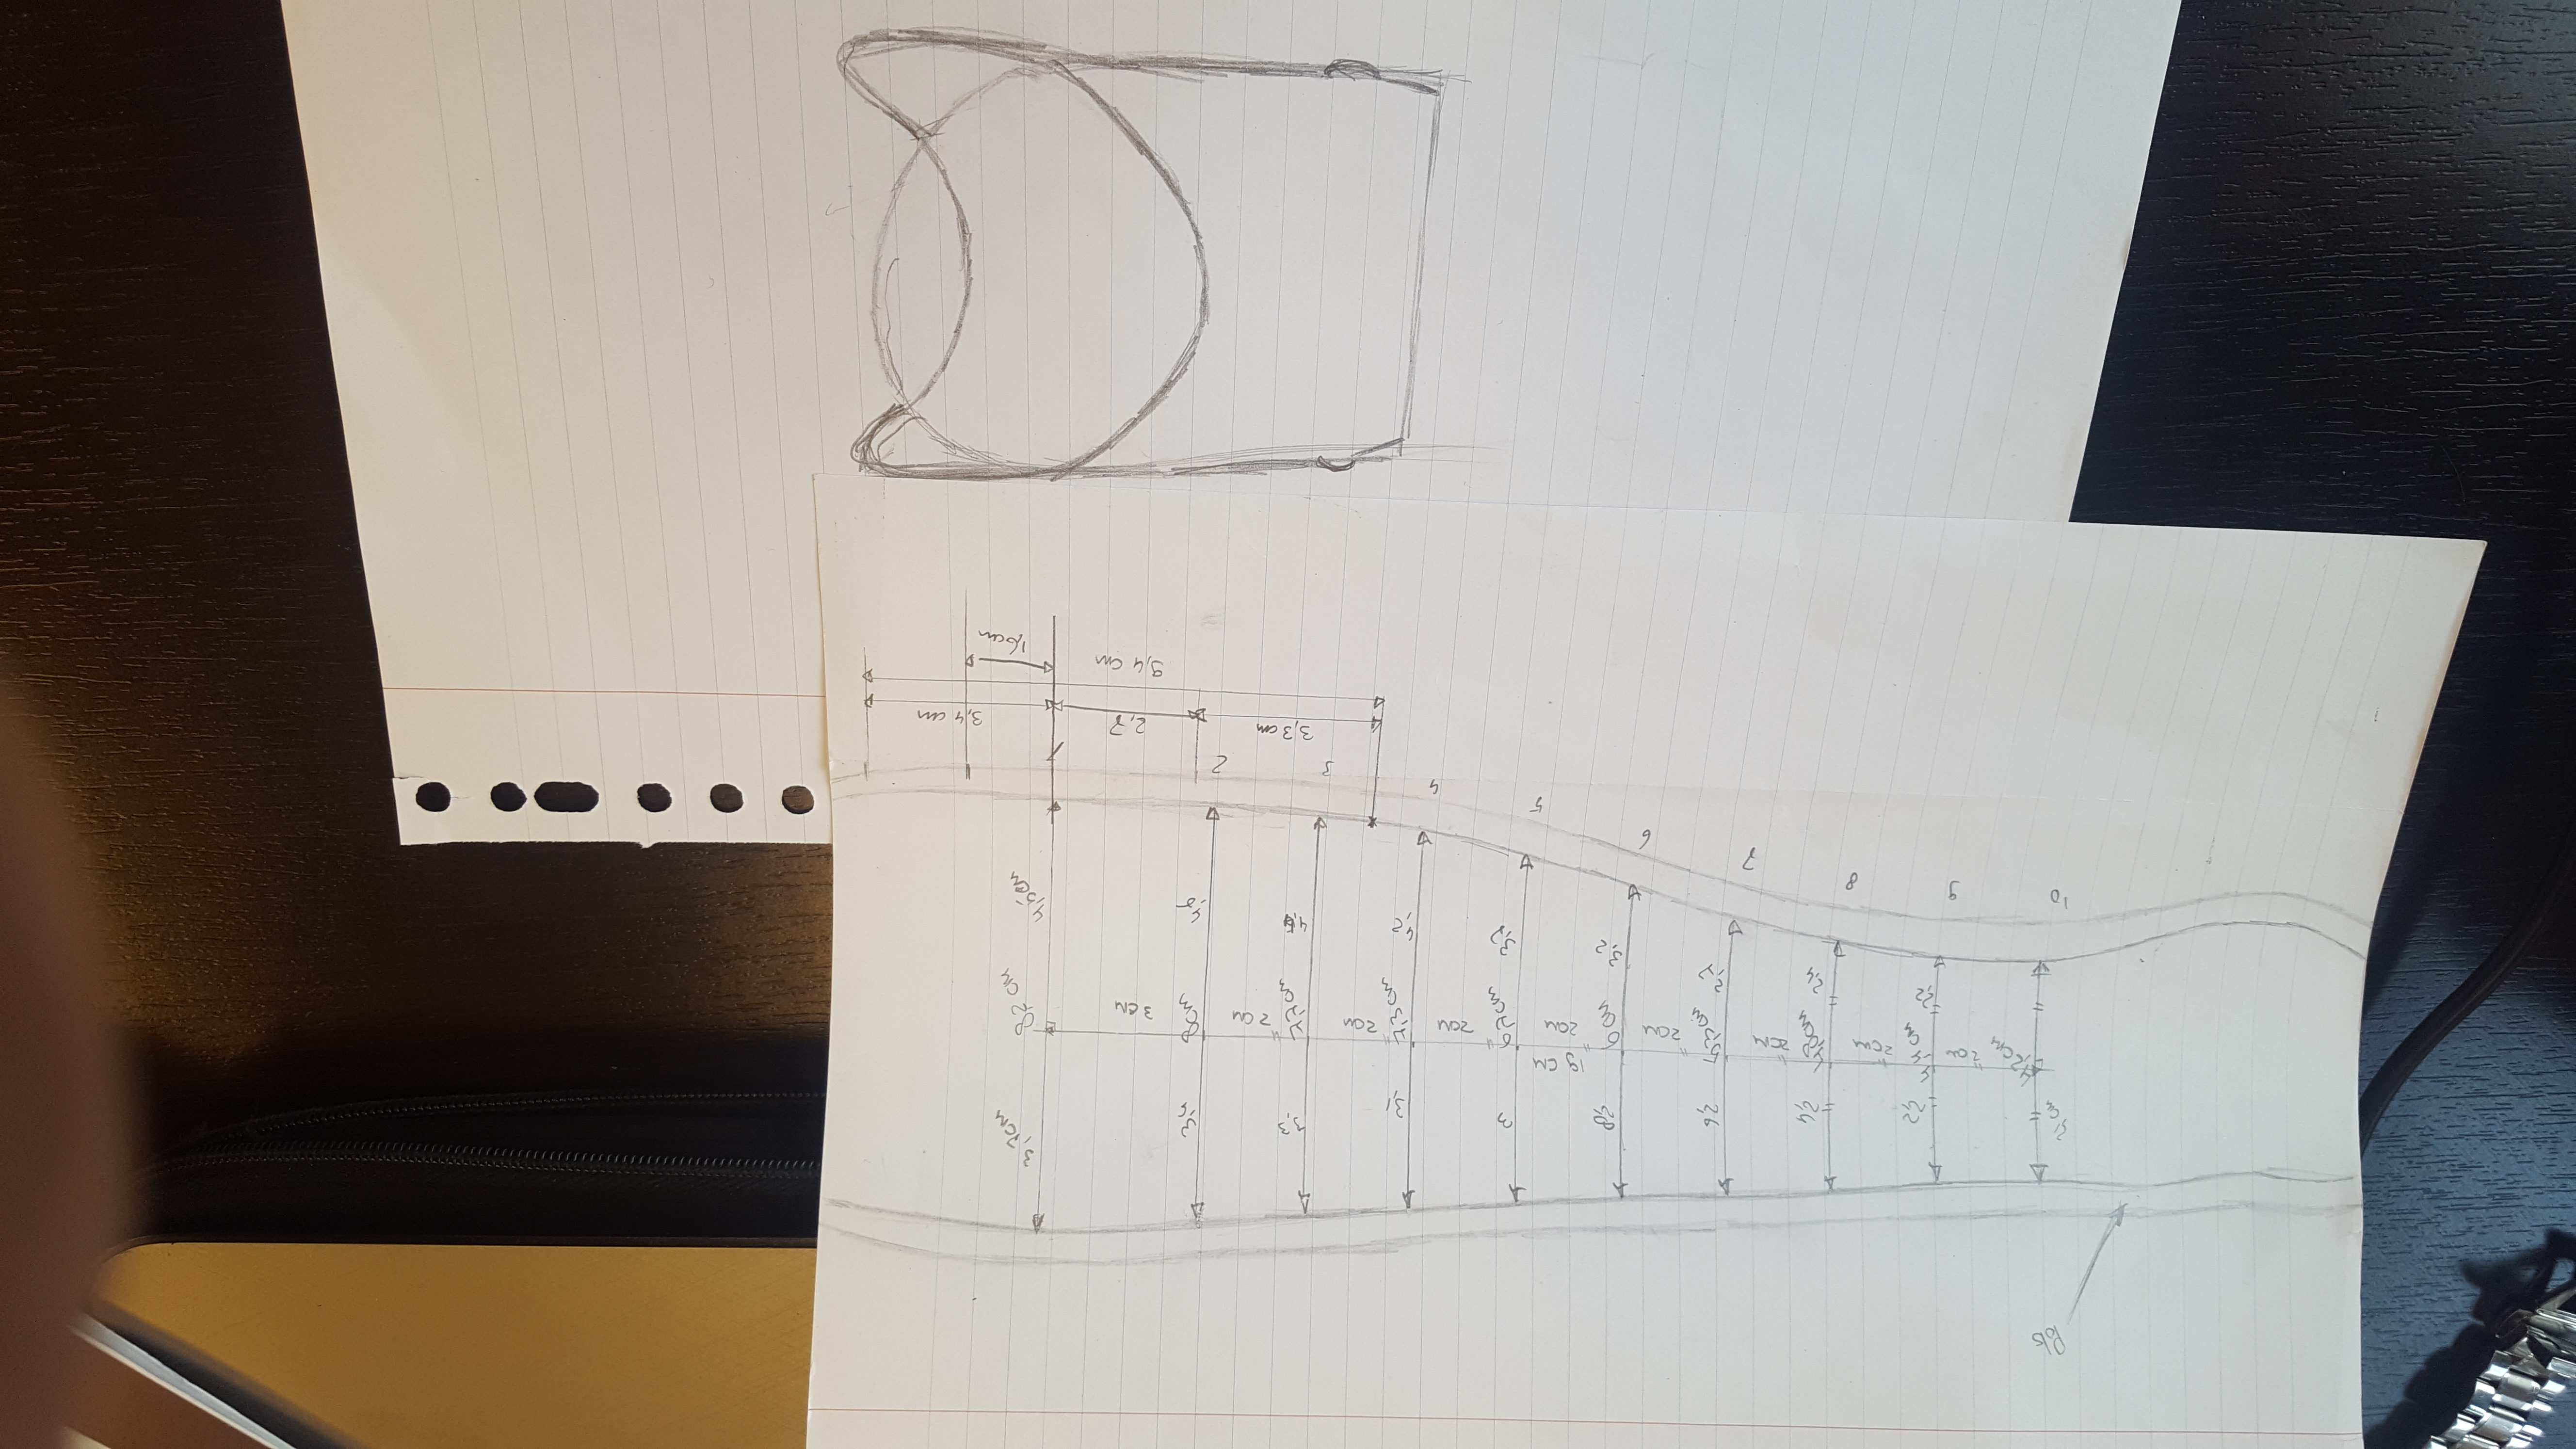
\includegraphics[scale=0.08, angle=180]{ConceptPrototype1.jpg}
    \caption{Concept drawings of the first prototype}
    \label{fig:ConceptPrototype1}
\end{figure} 

\newpage

\begin{landscape}
    \thispagestyle{empty}
    \begin{figure}[h]
        \centering
        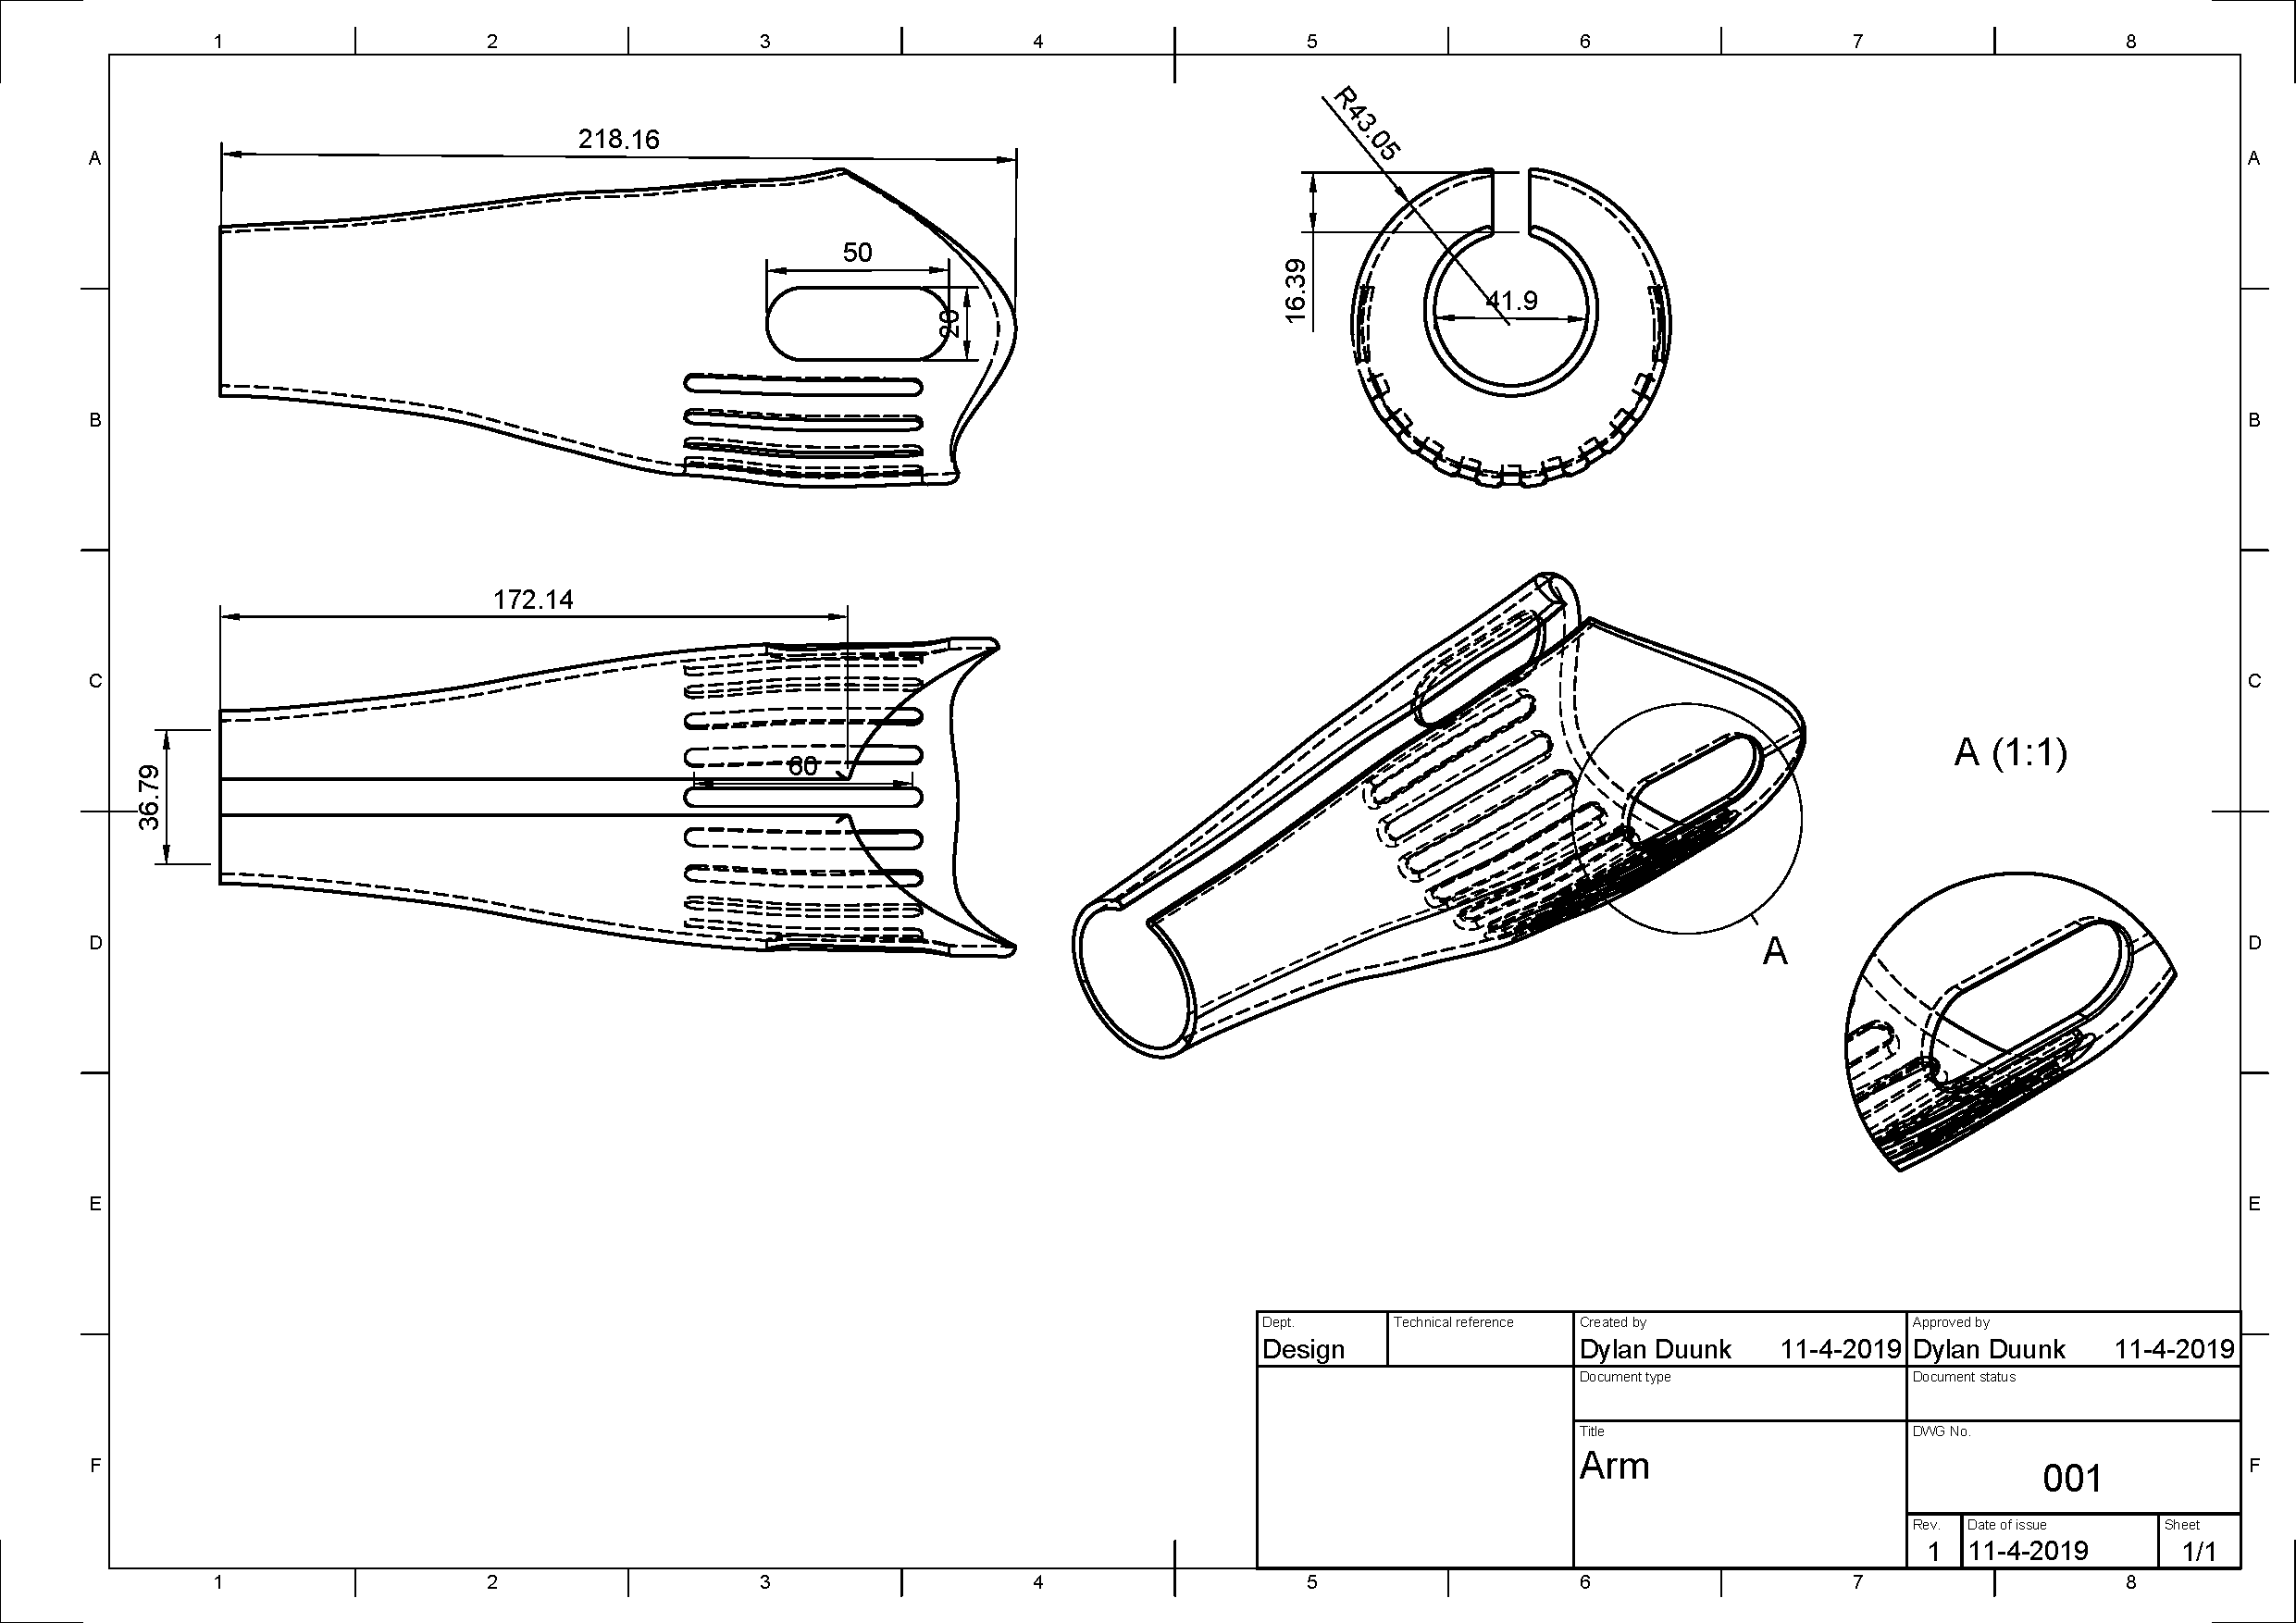
\includegraphics[scale=0.5]{Arm_Drawing_v3.pdf}
        \caption{Mechanical drawings for the first prototype. \textit{*Note: Measurements are mm!}}
        \label{fig:Prototype1Mechanical}
    \end{figure} 
\end{landscape}

\subsection{Second Prototype}
For the second prototype I wanted to make a casing specifically for my hand.
See figure \ref{fig:ConceptPrototype2} for my concept drawings. 
I moddeled around pictures of my hand in Fusion 360 and came up with this design (Figure \ref{fig:Prototype2Mechanical})
\\ \\
See table \ref{tab:SecondPrototypeProsCons} for the pros and cons of the second prototype.
\begin{table}[ht]
    \centering
    \begin{tabular}[t]{p{6cm} p{6cm}}
    \toprule
    \textbf{Pros} & \textbf{Cons} \\
    \midrule
    Thickness of the prototype is good. & Design is more suitable for users with a partial hand. \\
    Horizontal fit is good. & Vertical fit is in some places to loose. \\
    & Not designed for below-elbow and above-elbow amputees. \\ 
    \bottomrule
    \end{tabular}
    \caption{Second Prototype: Pros \& Cons}
    \label{tab:SecondPrototypeProsCons}
\end{table}

\begin{figure}[h]
    \centering
    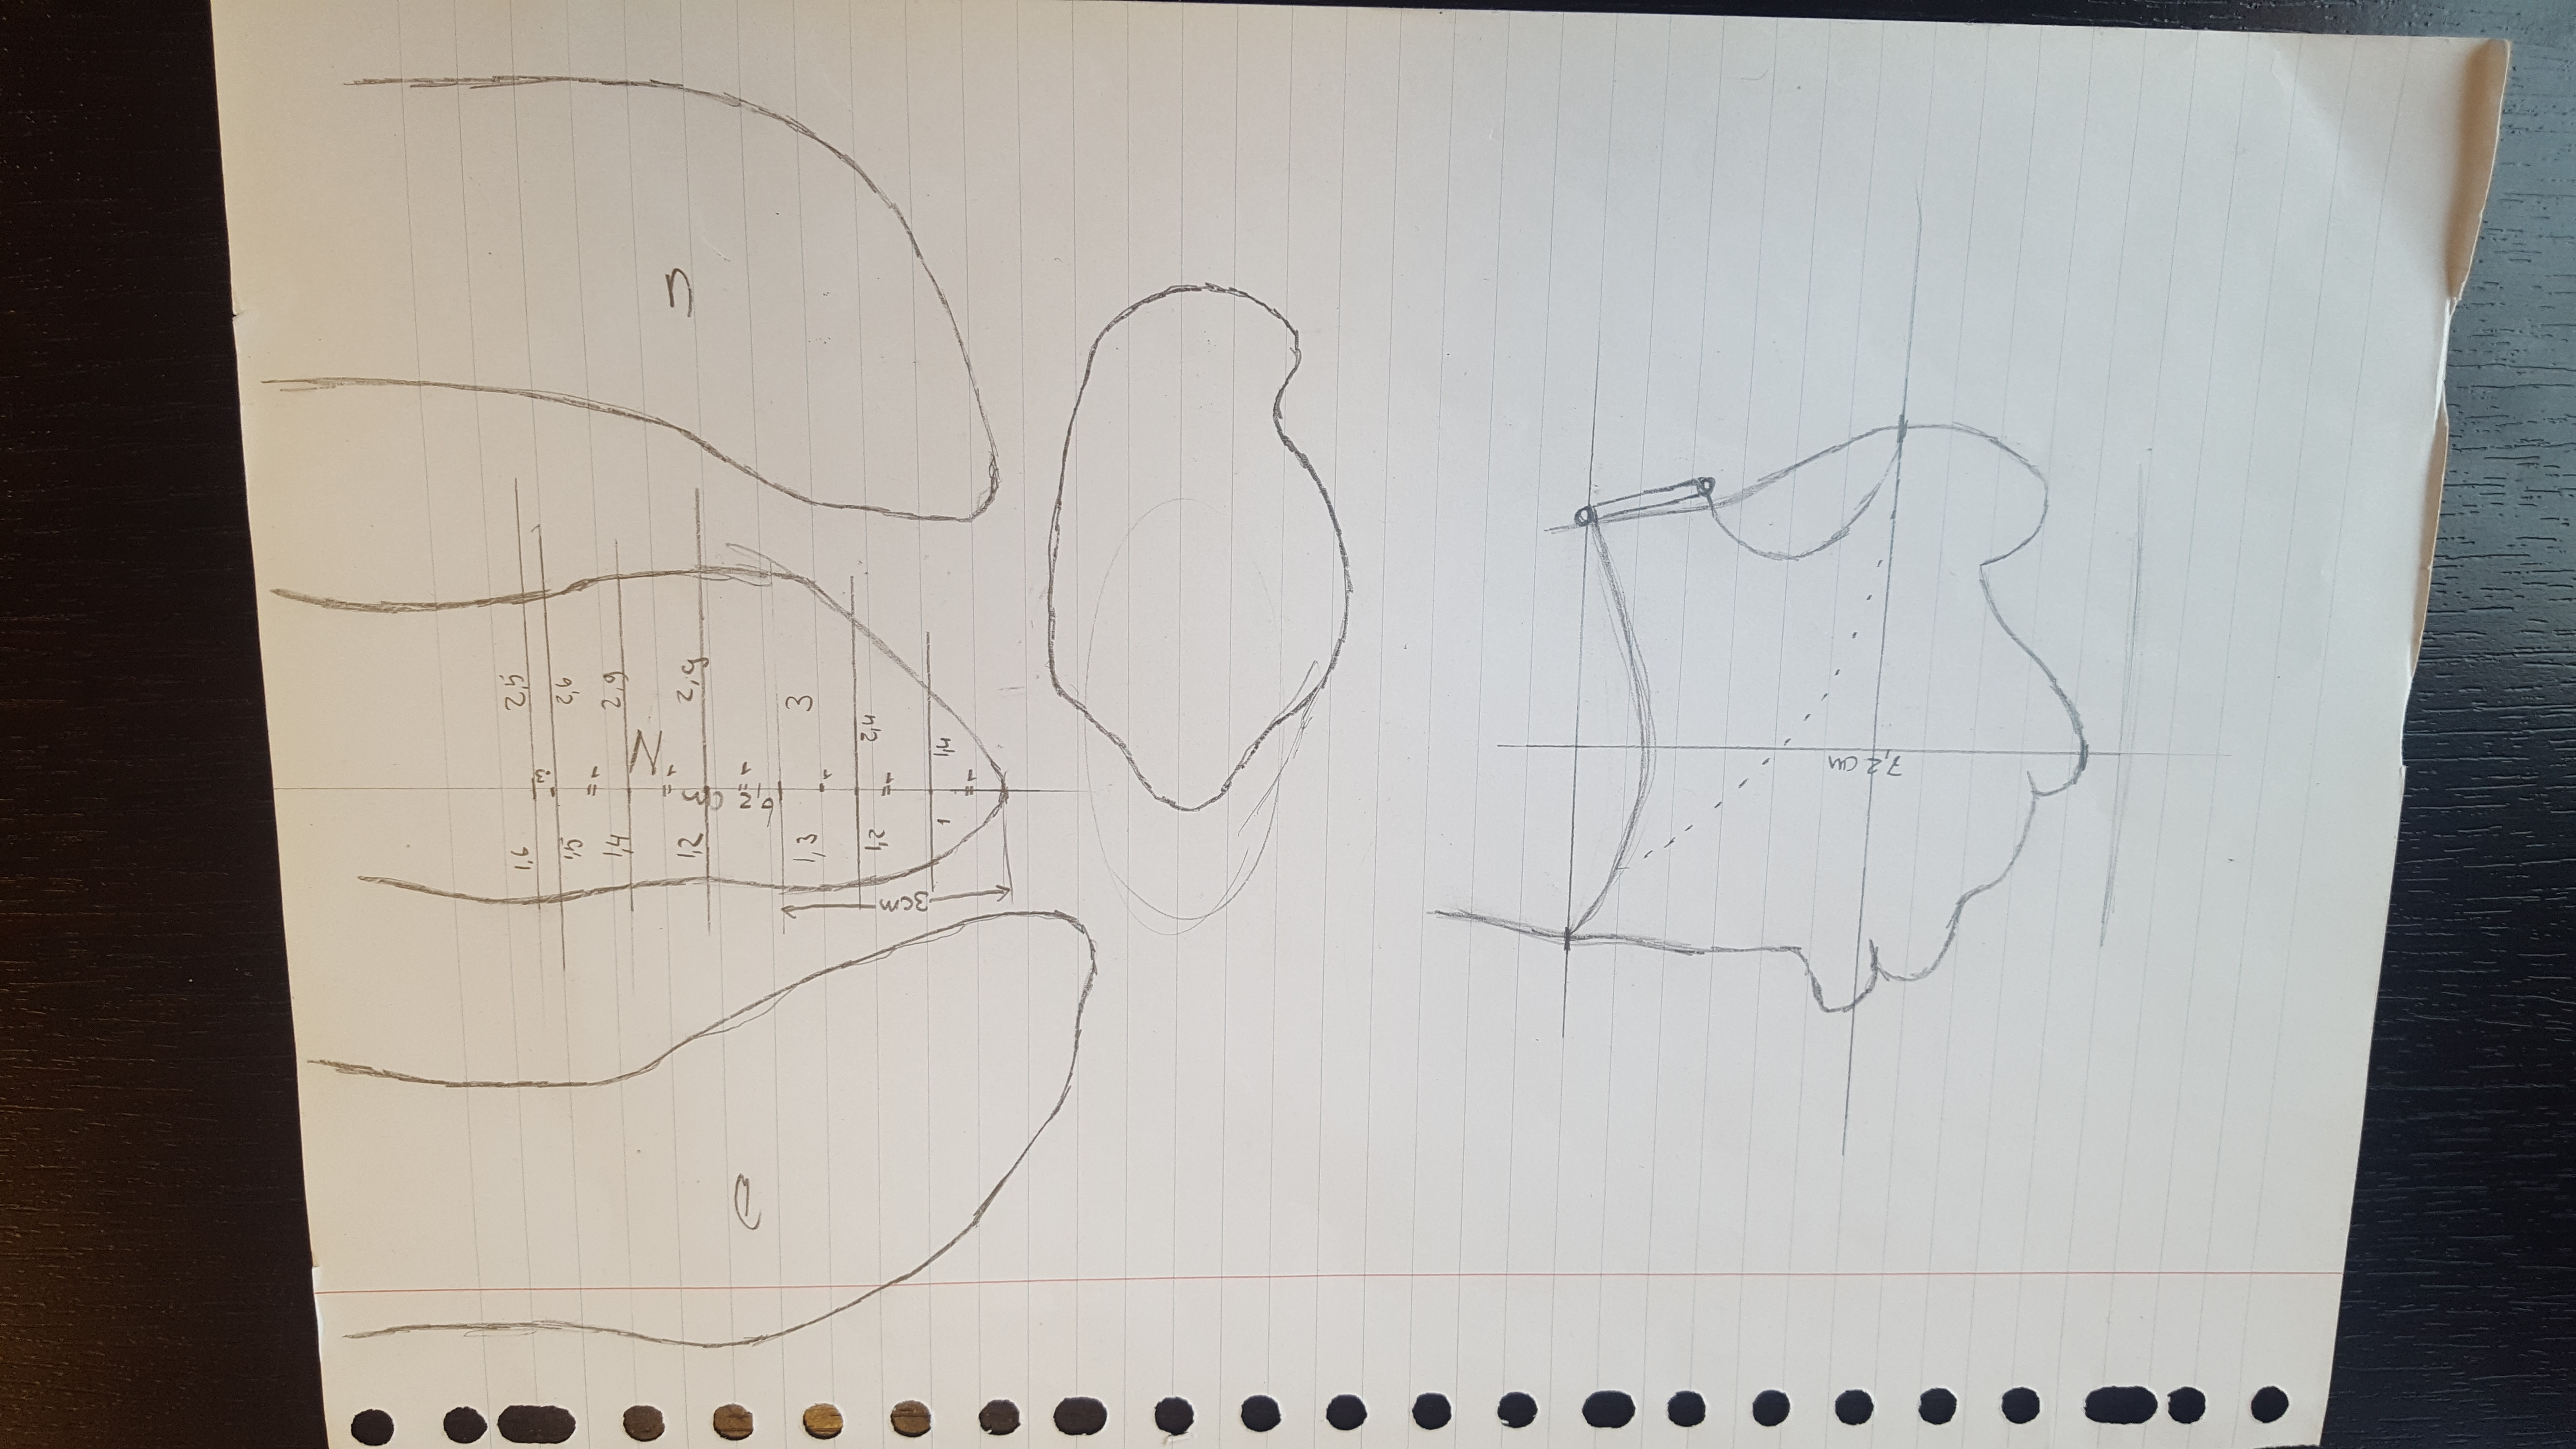
\includegraphics[scale=0.08, angle=180]{ConceptPrototype2.jpg}
    \caption{Concept drawings of the second prototype}
    \label{fig:ConceptPrototype2}
\end{figure} 

\newpage

\begin{landscape}
    \thispagestyle{empty}
    \begin{figure}[h]
        \centering
        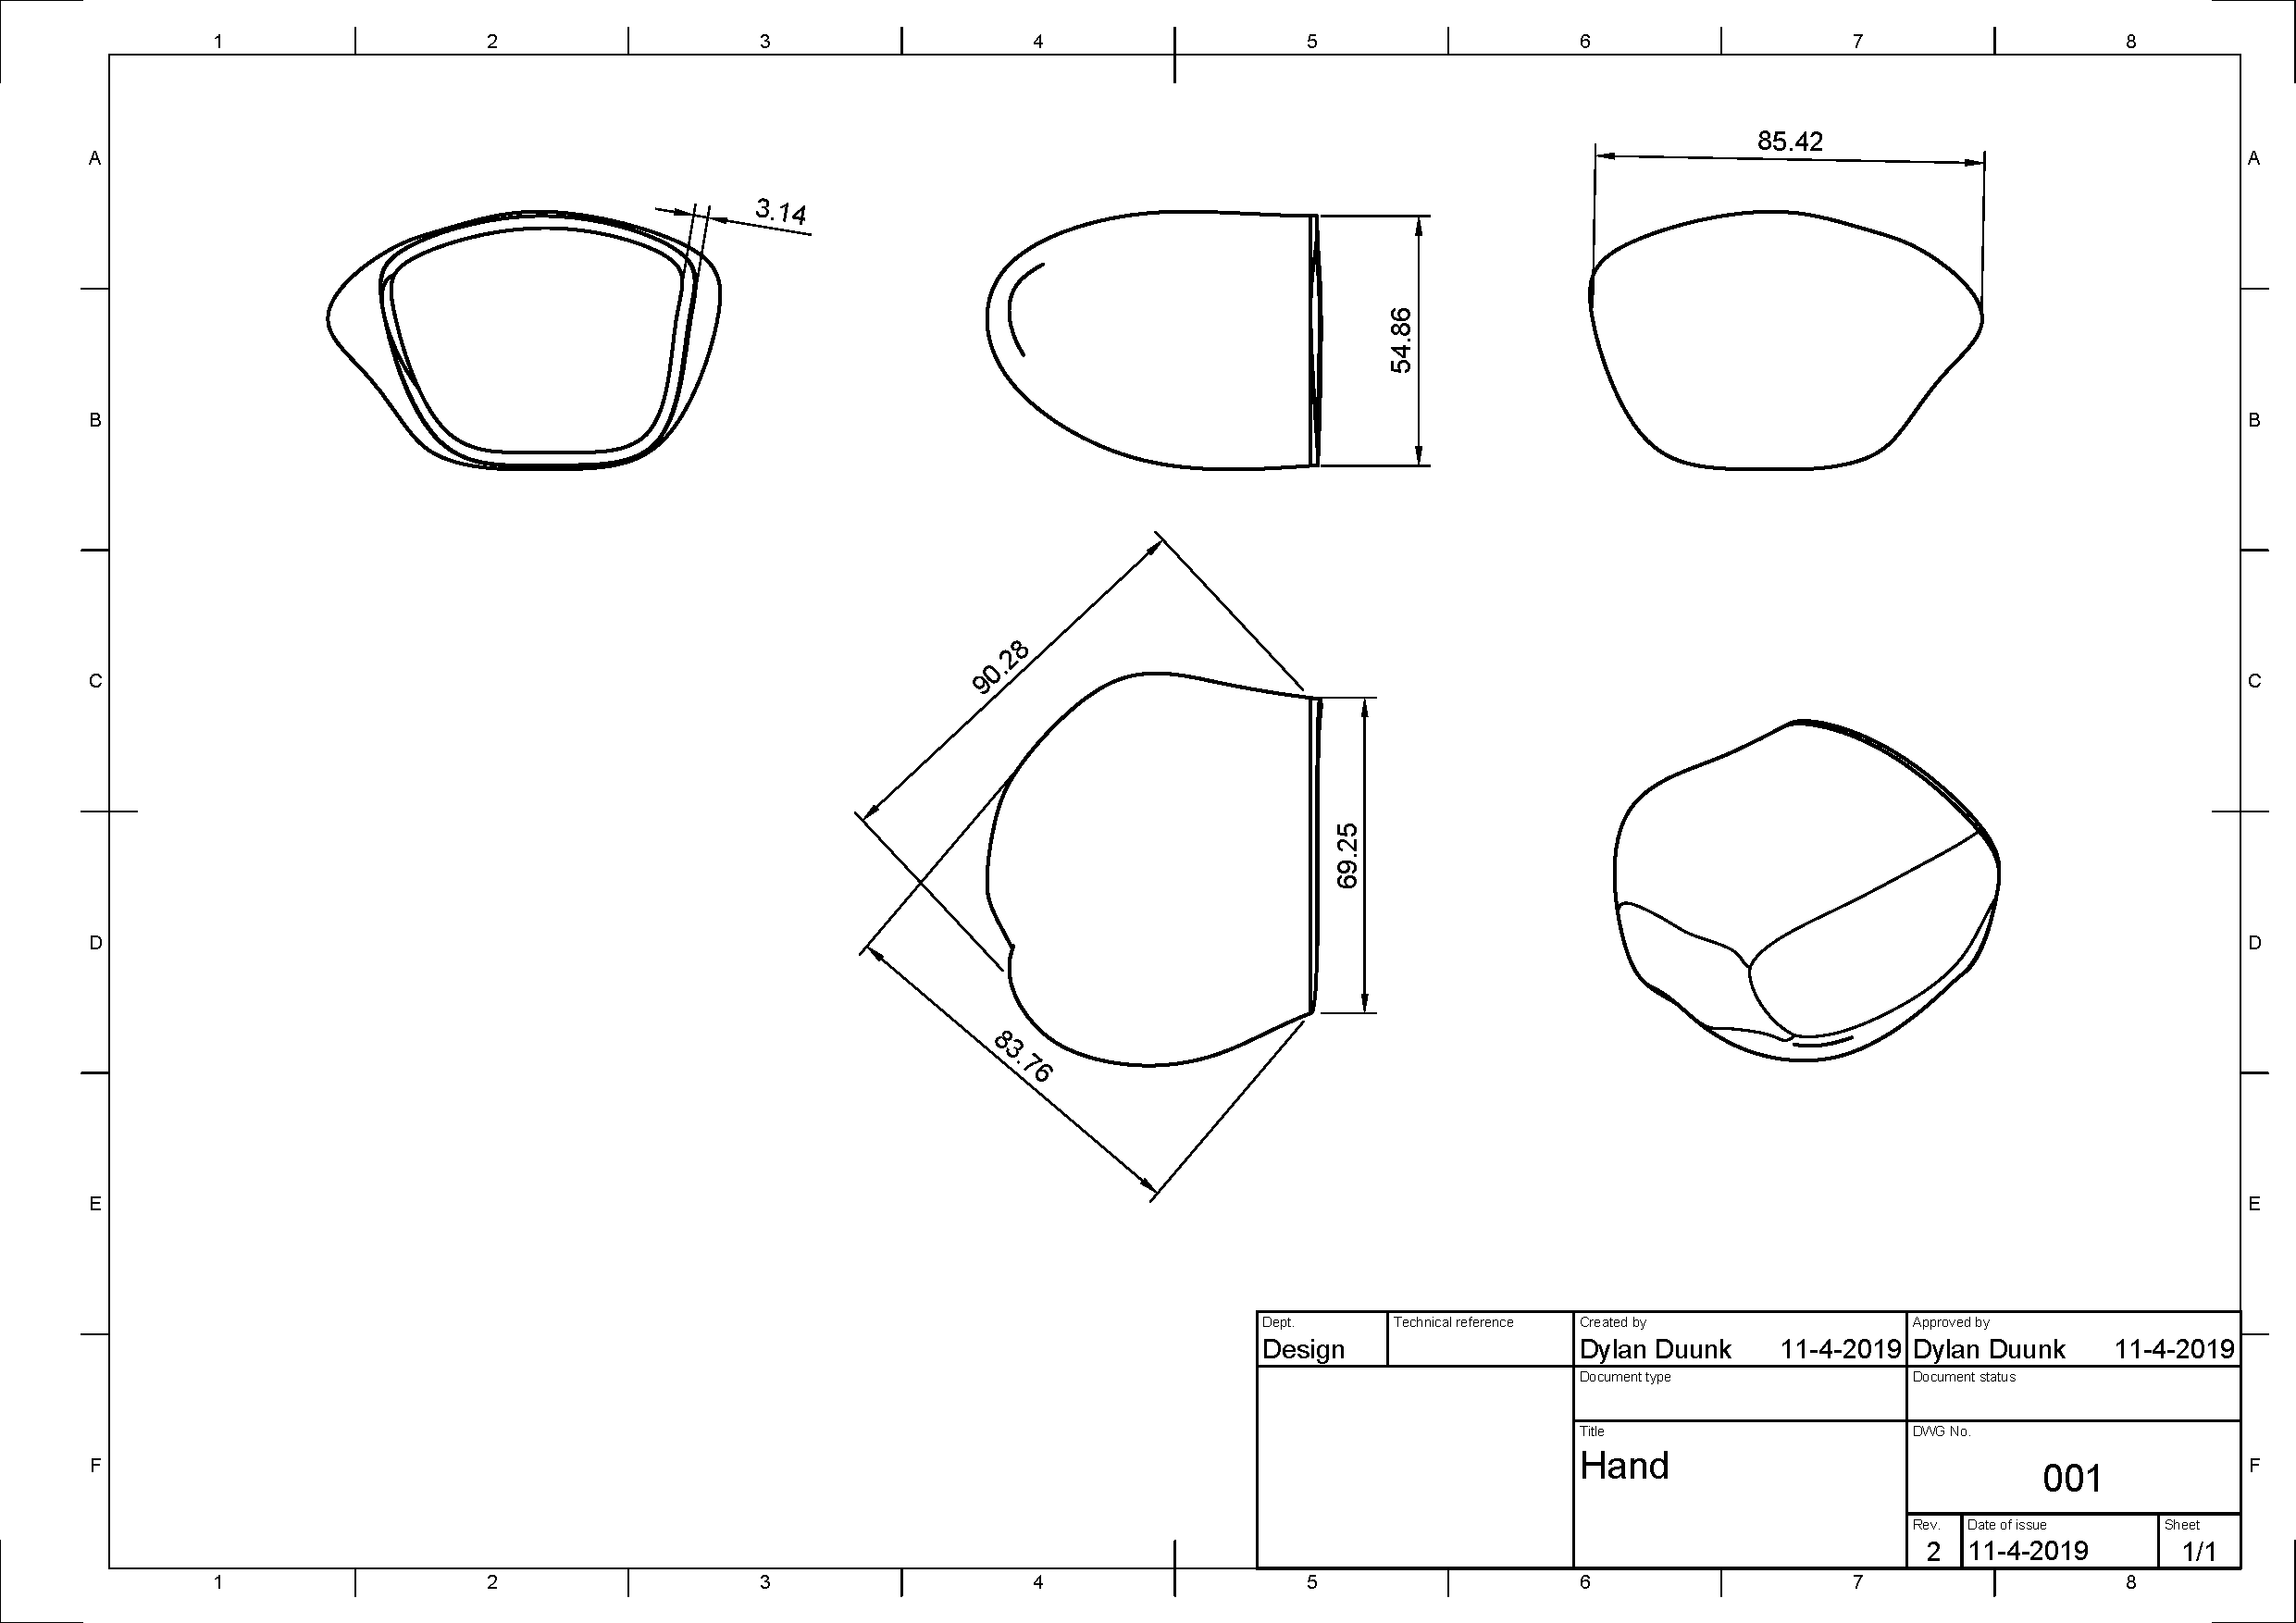
\includegraphics[scale=0.5]{Hand_Drawing_v1.pdf}
        \caption{Mechanical drawings for the second prototype. \textit{*Note: Some dimmensions could not be given and measurements are mm!}}
        \label{fig:Prototype2Mechanical}
    \end{figure} 
\end{landscape}

\subsection{Third Prototype}
For the third prototype I adjusted the fit of the second prototype and added a cutout so my hand could easily slide in .
I came up with this design (Figure \ref{fig:Prototype3Mechanical}).
\\ \\
See table \ref{tab:ThirdPrototypeProsCons} for the pros and cons of the third prototype.
\begin{table}[ht]
    \centering
    \begin{tabular}[t]{p{6cm} p{6cm}}
    \toprule
    \textbf{Pros} & \textbf{Cons} \\
    \midrule
    Thickness of the prototype is good. & A little cutout at the wrist would be nice. \\
    Fit is perfect. & Not designed for below-elbow and above-elbow amputees. \\ 
    No sharp edges. & \\
    Cutout is good. & \\
    \bottomrule
    \end{tabular}
    \caption{Third Prototype: Pros \& Cons}
    \label{tab:ThirdPrototypeProsCons}
\end{table}

\newpage

\begin{landscape}
    \thispagestyle{empty}
    \begin{figure}[h]
        \centering
        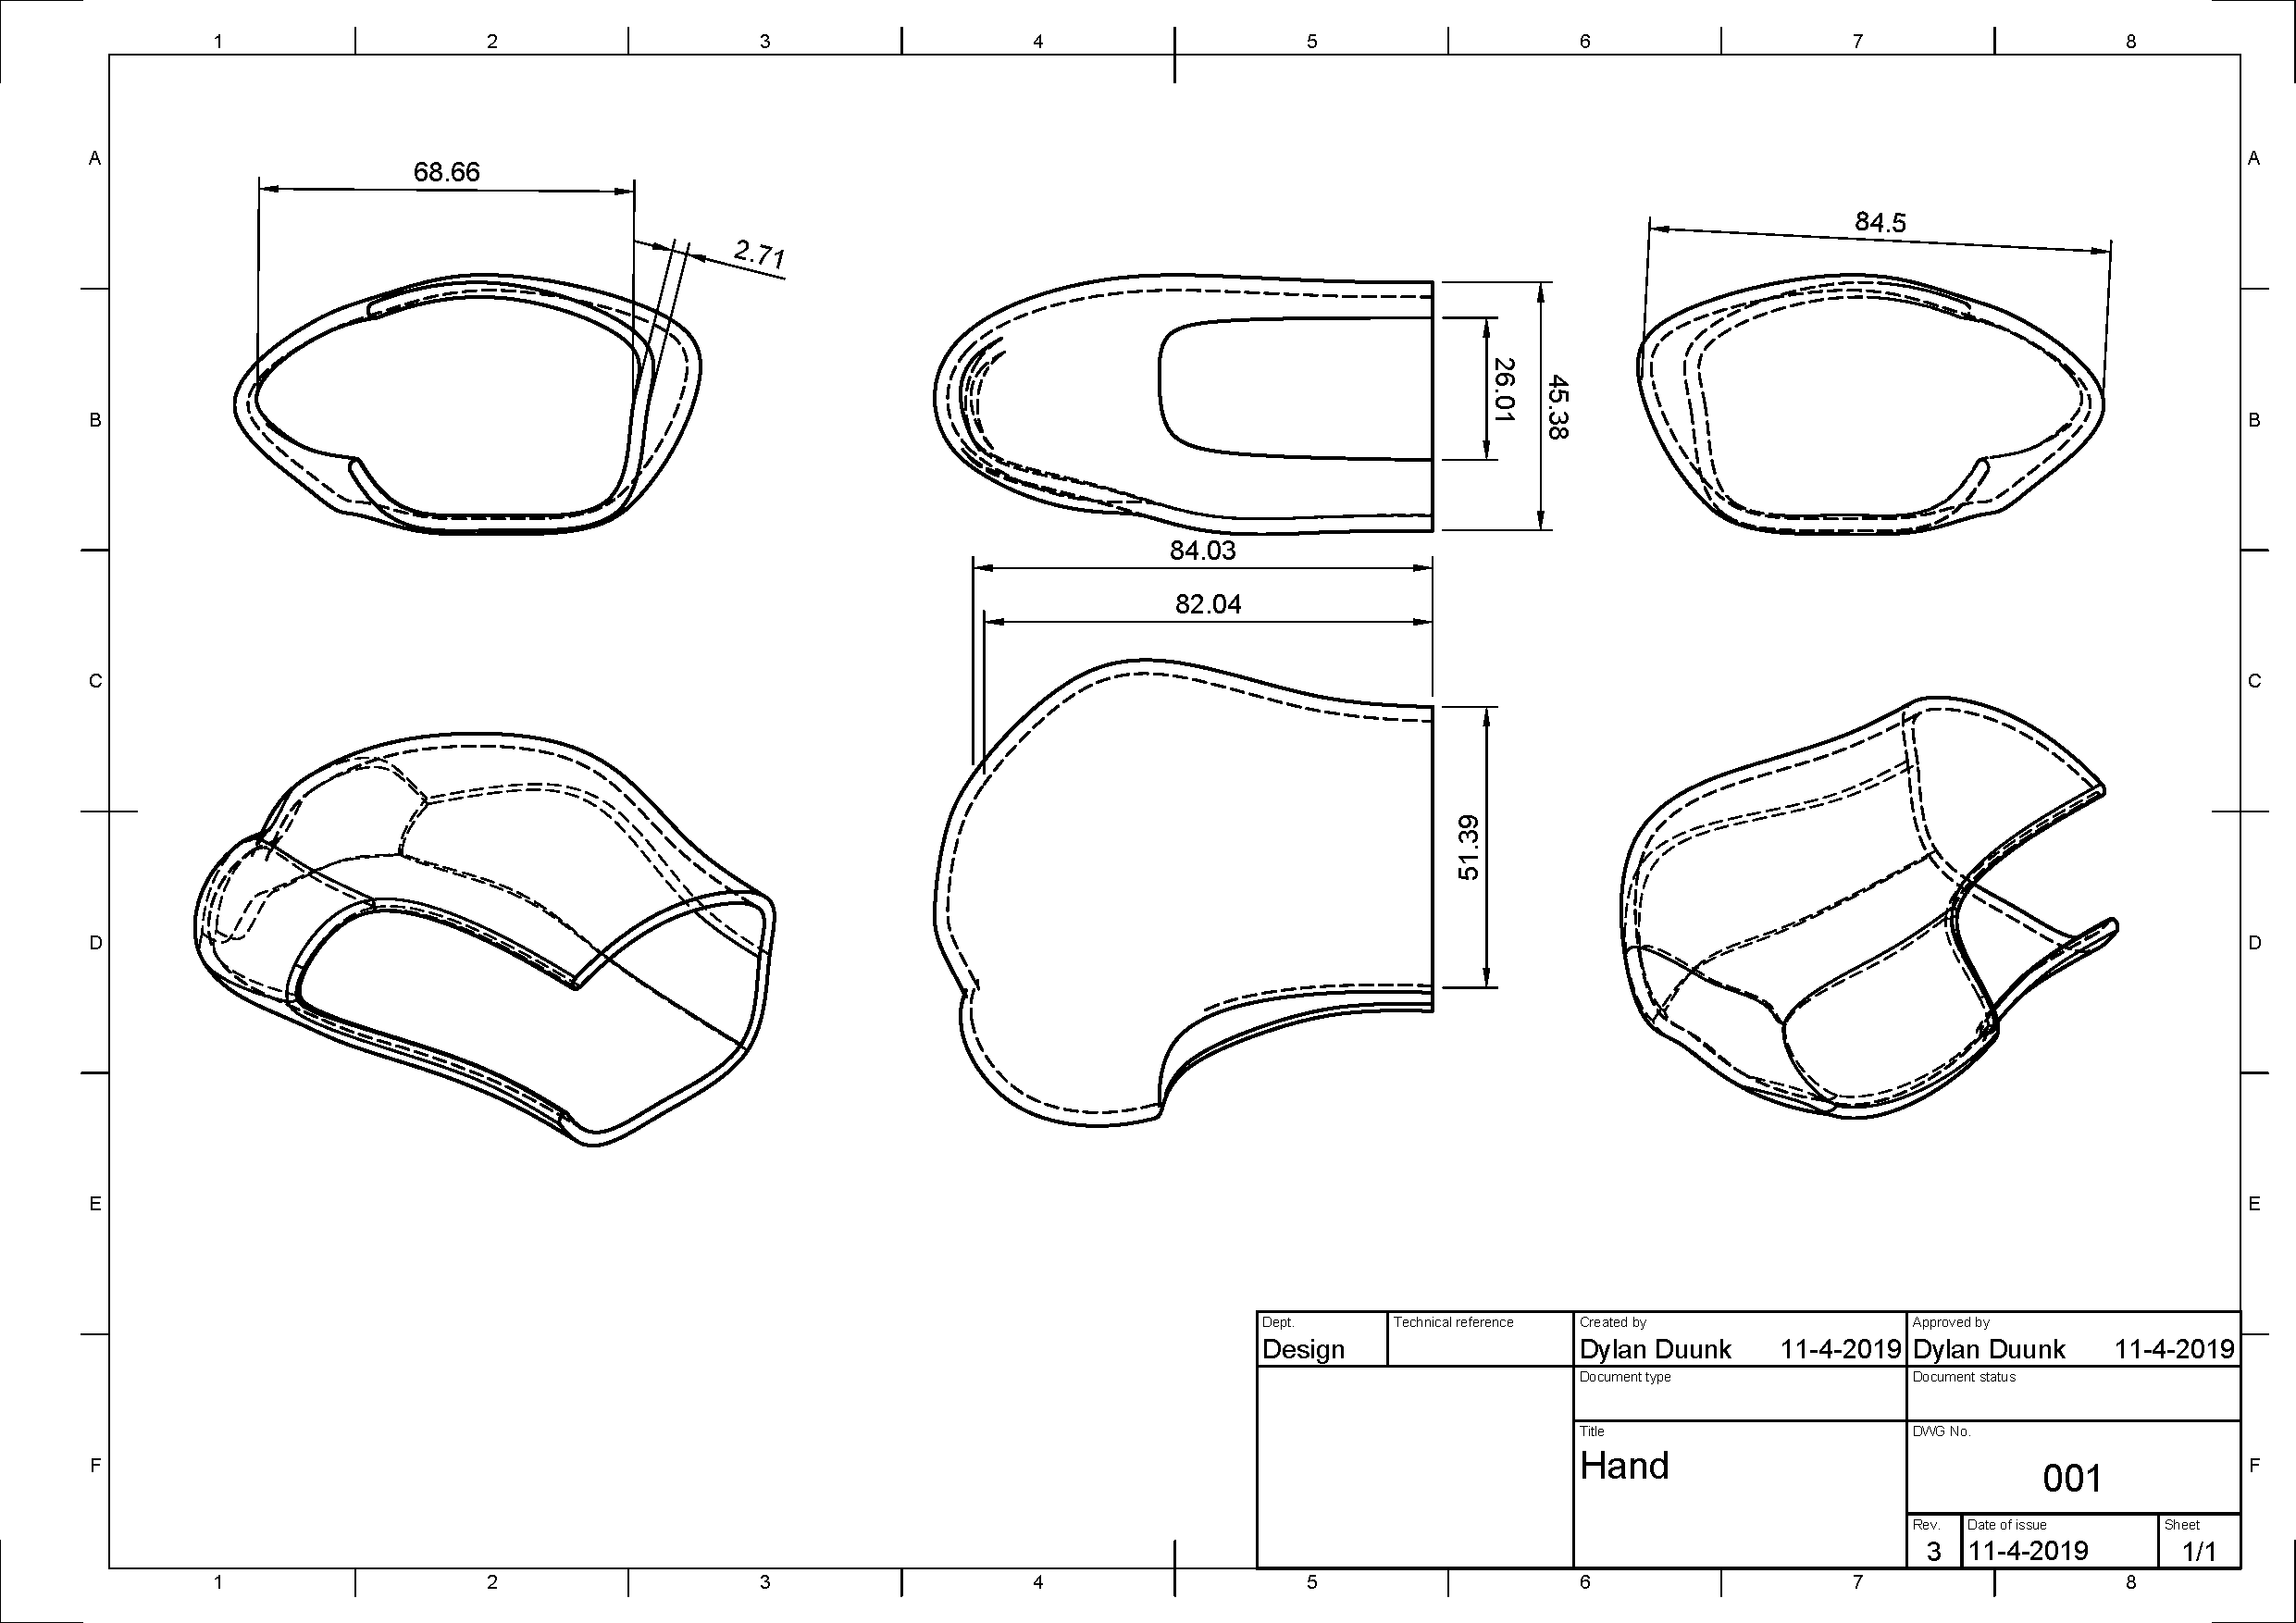
\includegraphics[scale=0.5]{Hand_Drawing_v2.pdf}
        \caption{Mechanical drawings for the third prototype. \textit{*Note: Some dimmensions could not be given and measurements are mm!}}
        \label{fig:Prototype3Mechanical}
    \end{figure} 
\end{landscape}

\newpage

\section{Conclusion and advice}

\subsection{Material}
A combination of PLA, ABS and Silicone would be the best choice material wise. 
This is because PLA and ABS are easy to use for rapid prototyping, in a relatively short time we can put together a functional prototype.
When further developing this prototype to a product i suggest to look into replacing parts with stronger materials.
When it comes to silicone, silicone is very suitable for the grip pads.
These pads make it easier to pick up objects.

\subsection{Comfort}
These are my recommendations for improving the comfort of our prototype:
\begin{description}[align=left]
    \item[Weight] See section Materials \ref{materials} for my recommendation about materials and weight.
                  Another way to minimize weight is by using light weight electrical components. 
    \item[Range of motion] All moveable parts in the prototype should be able to move freely.
                           These parts shouldn't restrict the movements that the user has without the prosthesis.  
    \item[Fit] Make the prototype fit the users arm by giving a almost perfect fit.
    \item[Breathability] This is done by giving the part that fits the users arm some breathing holes, whilst not compromising structural integrity.
    \item[Aesthetics] This is done by keeping the design simple and modern.
\end{description}

\subsection{Prototype Design}
My recommendations for other amputees:
\textit{*Note: this does not include the general shape, because my hand isa different size.}
\begin{description}
    \item[Above-elbow] Extend the first prototype design to the upper arm.
                       Make sure the prototype can be rotated where the elbow would have been.
                       If the fit at the upper arm is not good enough maybe look into attaching the prototype to the shoulder.
    \item[Below-elbow] Extend the first prototype aswell.
                       If the fit at the lower arm is not good enough maybe look into attaching the prototype to the elbow/upper arm.
    \item[Other partial hands] For people with no fingers or "little stumps" see my recommendations for extending the current design below.
                               For people with some fingers extend the third design by cutting holes for the existing fingers.  
\end{description}

My recommendations for extending the current design are:
\begin{itemize}
    \item Extend the third prototype with a palm.
    \item Extend the palm with a connection to the fingers.
    \item Make an extension to the wrist for extra stability.
\end{itemize}

\clearpage
\addcontentsline{toc}{section}{References}
\bibliography{literature}

\end{document}